\documentclass{LMCS}

\def\dOi{10(1:8)2014}
\lmcsheading {\dOi}
{1--20}
{}
{}
{Jan.~13, 2013}
{Feb.~12, 2014}
{}

\subjclass{F.4.3 Formal Languages}

\ACMCCS{[{\bf Theory of computation}]: Formal languages and automata
  theory---Automata extensions}





\usepackage {amsfonts}
\usepackage {amssymb,amsmath,amsthm}
\usepackage {tikz}






\usepackage {xspace}
\usepackage {url}

\usepackage{hyperref}

\usepackage {tikz}

\usetikzlibrary{positioning}
\usetikzlibrary{decorations.pathreplacing}
\usetikzlibrary{automata,positioning}
\usetikzlibrary{decorations.pathmorphing}
\usetikzlibrary{decorations.markings}
\usetikzlibrary{arrows}





\newcommand{\parnote}[2]{\vspace{10pt}\textcolor{#1}{\bf #2}\vspace{10pt}}


\newcommand{\myname}{Micha{\l} Skrzypczak}

\newcommand{\thanksosna}{\thanks{Author supported by ERC Starting Grant "Sosna" no. 239850}}

\newcommand{\thankslawek}{\thanks{This paper has been partially supported by the Polish Ministry of
Science grant no. N206 567840}}



\hyphenation{}



\newcommand{\operator}[2]{\newcommand{#1}{{{\ensuremath{\mathop{\mathrm{#2}}}\xspace}}}}



\newcommand{\domain}[2]{\newcommand{#1}{\ensuremath{\mathbb {#2}}}\xspace}



\newcommand{\qU}{\ensuremath{\mathsf U}\xspace}

\operator{\fo}{FO}
\operator{\mso}{MSO}
\operator{\wmso}{WMSO}
\operator{\msou}{MSO+U}
\operator{\wmsou}{WMSO+U}
\operator{\wmsor}{WMSO+R}
\newcommand{\wmsour}{Weak MSO \!+\textsf{U}+\textsf{R}\xspace}

\newcommand{\wBS}{\ensuremath{\omega \mathrm{BS}}\xspace}
\newcommand{\wB}{\ensuremath{\omega \mathrm{B}}\xspace}
\newcommand{\wS}{\ensuremath{\omega \mathrm{S}}\xspace}

\newcommand{\wT}{\ensuremath{\omega \mathrm{T}}\xspace}

\newcommand{\fT}{\ensuremath{\mathrm{T}}\xspace}
\newcommand{\fB}{\ensuremath{\mathrm{B}}\xspace}
\newcommand{\fS}{\ensuremath{\mathrm{S}}\xspace}



\domain{\N}{N}
\domain{\Z}{Z}
\domain{\Q}{Q}
\domain{\R}{R}
\domain{\C}{C}

\newcommand{\closure}{\mathrm{Closure}}

\newcommand{\prom}[1]{\ensuremath{\widehat{{#1}^\ast}}\xspace}

\newcommand{\aut}[1]{\ensuremath{\mathcal {#1}}\xspace}



\newcommand{\mathbold}[3]{\ensuremath{\mathbf{#1}^{#2}_{#3}}}

\newcommand{\borel}{\ensuremath{\mathcal B}\xspace}

\newcommand{\bsigma}[1]{\mathbold{\Sigma}{0}{#1}}
\newcommand{\bpi}[1]{\mathbold{\Pi}{0}{#1}}
\newcommand{\bdelta}[1]{\mathbold{\Delta}{0}{#1}}

\newcommand{\asigma}[1]{\mathbold{\Sigma}{1}{#1}}
\newcommand{\api}[1]{\mathbold{\Pi}{1}{#1}}
\newcommand{\adelta}[1]{\mathbold{\Delta}{1}{#1}}

\newcommand{\bc}[1]{\mathcal{BC}({#1})}



\newcommand{\comment}[1]{}



\newcommand{\fun}[3]{\ensuremath{#1\colon #2 \to #3}}
\newcommand{\parfun}[3]{\ensuremath{#1\colon #2 \rightharpoonup #3}}

\operator{\dom}{dom}
\operator{\id}{id}
\operator{\sgn}{sgn}



\operator{\close}{cl}
\operator{\inter}{int}

\newcommand{\restr}{\!\upharpoonright}

\newcommand{\newton}[2]{\ensuremath{\binom{#1}{#2}}}

\newcommand{\comp}[1]{\ensuremath{\overline{#1}}}

\newtheorem{test_thereom}{Test theorem}[section]

\newcommand{\newthm}[2]{\newtheorem{#1}[test_thereom]{#2}}

\newcommand{\ident}[2]{\newcommand{#1}{\ensuremath{\mathrm{#2}}\xspace}}

\ident{\lang}{L}



  \newthm{theorem}{Theorem}
  \newthm{lemma}{Lemma}
\newthm{definition}{Definition}
  \newthm{problem}{Problem}
  \newthm{proposition}{Proposition}
  \newthm{example}{Example}
  \newthm{corollary}{Corollary}
  \newthm{claim}{Claim}

  \newthm{observation}{Observation}
  \newthm{remark}{Remark}
  \newthm{assignment}{Assignment}
  \newthm{conjecture}{Conjecture}
  \newthm{note}{Note}



\title
[Separation property for \wB- and \wS-regular languages]
{Separation property for \wB- and \wS-regular languages}


\newcommand{\thankncn}{\thanks{Work supported by the National Science Center (decision 
DEC-2012/07/D/ST6/02443)}}

\author{Micha{\l} Skrzypczak}
\thankncn
\address{Institute of Informatics, University of Warsaw, ul. Banacha 2, 02-097 Warsaw, Poland}
\email{mskrzypczak@mimuw.edu.pl}
\keywords{-regular languages, counter automata, profinite monoid, \wS-regular languages}




\newcommand{\trans}[1]{\overset{#1}{\longrightarrow}}

\newcommand{\ceps}{\ensuremath{\mathbf{nil}}}
\newcommand{\cinc}{\ensuremath{\mathbf{inc}}}
\newcommand{\cres}{\ensuremath{\mathbf{reset}}}

\newcommand{\cop}{o}

\renewcommand{\setminus}{-}

\operator{\traces}{traces}

\operator{\sep}{sep}

\newcommand{\types}[1]{\ensuremath{\mathrm{Tp}^{#1}}\xspace}

\newcommand{\mcounter}{M_{\mathrm{counter}}}
\newcommand{\mtraces}{M_{\mathrm{trans}}}

\newcommand{\val}[1]{\mathrm{val}({#1})}

\newcommand{\shl}{\leftarrow}
\newcommand{\shr}{\rightarrow}

\newcommand{\finA}{w}
\newcommand{\finB}{z}
\newcommand{\seqA}{W}
\newcommand{\seqB}{Z}
\newcommand{\seqC}{Y}
\newcommand{\infA}{u}
\newcommand{\infB}{v}

\newcommand{\etype}{\mathrm{Etp}}



\begin{document}



\begin{abstract}
\noindent In this paper we show that \wB- and \wS-regular languages satisfy the following separation-type theorem
\begin{quote}
If  are disjoint languages of -words both recognised
by \wB- (resp. \wS)-automata then there exists an -regular
language  that contains , and whose complement contains .
\end{quote}

In particular, if a language and its complement are recognised by \wB- (resp. \wS)-automata then the language is -regular.

The result is especially interesting because, as shown by Boja{\'n}czyk and Colcombet, \wB-regular languages are complements of \wS-regular languages. Therefore, the above theorem shows that these are two mutually dual classes that both have the separation property. Usually (e.g. in descriptive set theory or recursion theory) exactly one class from a pair  has the separation property.

The proof technique reduces the separation property for -word languages to profinite languages using Ramsey's theorem and topological methods. After that reduction, the analysis of the separation property in the profinite monoid is relatively simple. The whole construction is technically not complicated, moreover it seems to be quite extensible.

The paper uses a framework for the analysis of \fB- and \fS-regular languages in the context of the profinite monoid that was proposed by Toru{\'n}czyk.
\end{abstract}

\maketitle



\section{Introduction}

The classes of \wB- and \wS-regular languages are extensions of -regular languages proposed by Boja{\'n}czyk and Colcombet in~\cite{bojanczyk_bounds}. The idea is to define \emph{asymptotic} properties of -words. The standard example is the following \wB-regular language


The main technical contribution of~\cite{bojanczyk_bounds} is the following theorem.
\begin{theorem}[Theorem~4.1 in~\cite{bojanczyk_bounds}]\label{th:duality}
The complement of an \wB-regular language is effectively \wS-regular and vice versa.
\end{theorem}

In this paper we show that both these classes admit the separation property. In general, a class of languages  has the \emph{separation property} with respect to a class , if the following condition holds:

\begin{quote}
For every pair of disjoint languages  from  there exists a language  such that\footnote{To distinguish the complement from the closure we denote the complement of a set  by .}

\end{quote}

In that case we say that  \emph{separates}  and . If not mentioned otherwise, the class  is taken as .

Usually, one class from a pair of dual classes  has the separation property and the other one does not. Below we recall some known separation-type theorems. The first one is a simple observation about Borel sets.

\begin{theorem}[Theorem~II~22.16 in~\cite{kechris_descriptive}]
Let . Every two disjoint  languages can be separated by a language that belongs to . On the other hand, there exists a pair of disjoint languages in  that cannot be separated as above.
\end{theorem}

The following theorem is an important extension to the projective hierarchy.

\begin{theorem}[Lusin (see~\cite{kechris_descriptive}]
If  are two disjoint analytic sets then there exists a Borel set separating them. There exists a pair of disjoint co-analytic (i.e. ) sets that cannot be separated by any Borel set.
\end{theorem}

The above theorem has its counterpart for regular languages of infinite trees. There is a correspondence between the parity index of a tree automaton and the topological complexity of the tree-language recognised by it. In particular, alternating -parity tree automata (ATA) recognise analytic languages, -parity ATA recognise co-analytic sets, while weak alternating automata recognise only Borel languages. The following two theorems are analogous to the above one in the tree-regular context.

\begin{theorem}[Rabin~\cite{rabin_separation}, also Kupferman, Vardi~\cite{kupferman_complementation}]\label{th:rabin_sep}
If  are two disjoint regular tree languages recognised by -parity ATA then there exists a language separating them recognisable by a weak alternating automaton (thus Borel).
\end{theorem}

\begin{theorem}[Hummel, Michalewski, Niwi{\'n}ski~\cite{hummel_separation}]
There exists a pair of tree-languages recognised by -parity ATA that cannot be separated by any Borel set.
\end{theorem}

The above theorem is extended for higher levels of the alternating index hierarchy in~\cite{michalewski_separation}. Theorem~\ref{th:rabin_sep} relies on the fact that every alternating -parity tree automaton is equivalent to a nondeterministic -parity tree automaton.

In this work we show that both classes of \wB- and \wS-regular languages have the separation property with respect to -regular languages. The proposed constructions are effective. The result is especially interesting since these are two mutually dual classes (see Theorem~\ref{th:duality} above). As a consequence of the separation properties we obtain the following corollary.

\begin{corollary}
If a given language of -words  and its complement  are both \wB-regular (resp. \wS-regular) then  is -regular.
\end{corollary}

The above result in the case of \wB-regular languages was independently known by some researchers in the area. Nevertheless, to the best of the author's knowledge, it has never been published.

To prove the main result we reduce the separation property of -word languages to the case of profinite words. For this purpose we use \fB- and \fS-automata introduced in~\cite{colcombet_stabilisation}. As shown in~\cite{torunczyk_limitedness} it is possible to define a language recognised by a \fB- or \fS-automaton as a subset of the profinite monoid . An intermediate step in our reasoning is proving the separation property for \fB- and \fS-regular languages of profinite words.

The paper is organised as follows. In Section~\ref{s:basic} we introduce basic notions. Section~\ref{s:automata} defines the automata models we use. In Section~\ref{s:profinite_sep} we prove separation results for languages of profinite words recognised by \fB- and \fS-automata. Section~\ref{s:reduction} contains the crucial technical tool, Theorem~\ref{th:recognition}, that enables to transfer separation results for languages of profinite words to the case of -words. In Section~\ref{s:omega_sep} we use this theorem to show that \wB- and \wS-regular languages have the separation property. Section~\ref{s:direct} contains a direct and simpler proof of the separation property for the \wB-regular case. This proof was proposed by Thomas Colcombet, we present it here with his kind permission. Finally, in Section~\ref{s:ack} we give acknowledgements.



\section{Basic notions}\label{s:basic}

We work with two models (\wB and \wS) at the same time. Therefore, we introduce a notion \wT to denote one of the models: \wB or \wS. By \fT we denote the corresponding finite word automata (\fB or \fS). By  we denote a finite alphabet. Elements of  are called finite words while  is the set of -words.



\subsection{Monoids}

We use monoids and Ramsey's theorem to decompose -words into finite ones.

\begin{definition}
A (finite) \emph{monoid} is a (finite) algebraic structure  equipped with an operation  that is associative () and with a distinguished element  that satisfies .

The operation  is called \emph{product} and  is called the \emph{neutral element}.

An element  is called \emph{idempotent} if .
\end{definition}

Observe that the set of all finite words  has a natural structure of monoid with the operation of concatenation and  defined as the empty word.

\begin{definition}
A function  is a \emph{homomorphism} between monoids  if it preserves the product:

\end{definition}

Now we define the monoid representing possible \emph{runs} of a nondeterministic automaton. It can be seen as an algebraic formalisation of the structure used by B\"uchi~\cite{buchi_decision} in his famous complementation lemma.

\begin{definition}
Let  be a nondeterministic automaton with states . Define  as . Let the neutral element be  and product:


Let  map a given finite word  to the set of pairs  such that the automaton  has a run over  starting in  and ending in .
\end{definition}

It is easy to check that  is a finite monoid and  is a homomorphism.

\subsection{Profinite monoid}

In this subsection we introduce the profinite monoid . A formal introduction to profinite structures can be found in~\cite{almeida_profinite} or~\cite{pin_profinite}. We refer to~\cite{pin_profinite}.

First we provide a construction of the profinite monoid . The idea is to enhance the set of all finite words by some \emph{virtual} elements representing sequences of finite words that are more and more similar.

Let  be a list of all regular languages of finite words. Let . Each element  can be seen as a sequence of bits, the bit  indicates whether our \emph{virtual} word belongs to the language .

Define  by the following equation:


The function  defined above is an embedding of  into . Let  be the closure of  in  with respect to the product topology of . Therefore,  contains  and the limits of its elements. To simplify the notion we identify  with its image .

\begin{example}[Proposition~2.5 in~\cite{pin_profinite}]\label{ex:factorial}
Let  for . A simple automata-theoretic argument shows that for every regular language , either almost all words  belong to  or almost all do not belong to . Therefore, the sequence  is convergent coordinate-wise in . The limit of this sequence is an element of .
\end{example}

The following fact summarises basic properties of .

\begin{fact}[Proposition~2.1, Proposition~2.4, and Theorem~2.7 in~\cite{pin_profinite}]
 is a compact metric space.  (formally ) is a countable dense subset of .  has a structure of a monoid that extends the structure of  and the concatenation is continuous.
\end{fact}

It turns out that the operation assigning to every regular language of finite words  its topological closure  has good properties (see Theorem~\ref{th:iso}). Therefore, we introduce the following definition.

\begin{definition}
A \emph{profinite-regular} language is a subset of  of the form  for some regular language .
\end{definition}

Using this definition, we can denote a generic profinite-regular language as  for  ranging over regular languages. Using the definition of  one can show the following easy fact.

\begin{fact}\label{ft:coordinates}
A language of profinite words  is profinite-regular if and only if it is of the form

for some . In that case .
\end{fact}

The structures of profinite-regular and regular languages are in some sense identical. This is expressed by the following fact.

\begin{theorem}[Theorem~2.4 in~\cite{pin_profinite}]\label{th:iso}
The function  is an isomorphism of the Boolean algebra of regular languages and the Boolean algebra of profinite-regular languages. Its inverse is  (when identifying  with  we can write ).
\end{theorem}

By the definition of  and fact that regular languages are closed under finite intersection, we obtain the following important fact.

\begin{fact}\label{ft:basis}
The family of regular languages of profinite words is a basis of the topology of .
\end{fact}

The topology of  is the product topology. Therefore, a sequence of finite words  is convergent to  if and only if  is convergent coordinate-wise to . The following fact formulates this condition in a more intuitive way.

\begin{fact}\label{ft:conv_seq}
A sequence of finite words  is convergent to  if and only if for every profinite-regular language  either:
\begin{itemize}
\item  and almost all words  belong to ,
\item  and almost all words  do not belong to .
\end{itemize}
\end{fact}

The topology of  is defined in such a way that it corresponds precisely to profinite-regular languages. The following fact summarises this correspondence.

\begin{fact}[Proposition~4.2 in~\cite{pin_profinite}]\label{ft:clopen}
A language  is profinite-regular if and only if it is a closed and open (clopen) subset of .
\end{fact}

\begin{proof}
First assume that  is a regular language of profinite words. Equation \eqref{eq:coords} in Fact~\ref{ft:coordinates} defines a closed and open set.

Now assume that  is a closed and open subset of . Recall that profinite-regular languages form a basis for the topology of  (Fact~\ref{ft:basis}). Since  is open so it is a union of base sets . Since  is a closed subset of a compact space ,  is compact. Therefore, only finitely many languages among  form a cover of . But a finite union of profinite-regular languages is a profinite-regular language. Therefore,  is profinite-regular.
\end{proof}

\subsection{Ramsey-type arguments}

In this subsection we recall Ramsey's theorem and show its application to finite monoids. This technique was used by B\"uchi in his complementation lemma~\cite{buchi_decision}. Additionally, we recall some extensions of Ramsey's theorem to compact spaces. In the following, by  we denote the set of all unordered pairs of natural numbers.

\begin{theorem}[Ramsey]\label{th:ramsey}
Assume that  is a function that assigns to every pair of numbers  a \emph{colour} . Additionally, assume that the set of colours  is finite. Then there exists an infinite \emph{monochromatic} set : a set  such that for some colour  and every pair of numbers  we have

\end{theorem}

The following theorem shows an application of Ramsey's theorem to the -word case.

\begin{theorem}\label{th:ramsey_decomposition}
Let  be a finite monoid and  be a homomorphism. Then for every -word  there exists a sequence of finite words  and two elements  of the monoid  such that:
\begin{enumerate}[label=(\roman*)]
\item ,
\item ,
\item  for every ,
\item  and .
\end{enumerate}
\end{theorem}

A pair  satisfying the above constraints is often called a \emph{linked pair}, see~\cite{perrin_pin_words}. To simplify the properties in the above theorem we introduce the following definition.

\begin{definition}
For a given homomorphism  we say that the \emph{type} (or \emph{-type}) of a decomposition  is  if: , , , and  for all .
\end{definition}

Using the above definition we can restate Theorem~\ref{th:ramsey_decomposition} as: for every -word  and homomorphism  there exists some decomposition of  of some type . A priori there may be two decompositions of one -word of two distinct types.

There is an extension of finite-colour Ramsey's theorem to the case where colours form a compact metric space. To state it formally we use the following definitions.

\begin{definition}
Assume that  is a sequence of finite words. We say that  is a \emph {grouping} of  if there exists an increasing sequence of numbers  such that for every  we have

\end{definition}

Note that if  is a decomposition of an -word  and  is of -type  then every grouping of  is also a decomposition of  of -type . The notion of grouping introduces a stronger version of convergence.

\begin{definition}
We say that a sequence of finite words  is \emph{strongly convergent} to a profinite word  if every grouping of  is convergent to .
\end{definition}

The following result can be seen as a simple extension of the Ramsey theorem to the case of the profinite monoid.

\begin{theorem}[Boja{\'n}czyk, Kopczy{\'n}ski, Toru{\'n}czyk~\cite{bojanczyk_ramsey_compact}]\label{th:ramsey_compact}
Let  be an infinite sequence of finite words. There exists a grouping  of  such that  strongly converges in .
\end{theorem}

For the sake of completeness we give a proof of this fact below. The theorem holds in general, where instead of  is any compact metric monoid. Also, the notion of convergence can be strengthened in the thesis of the theorem: all the groupings of  converge in a \emph{uniform way}. In this paper we use only the above, simplified form.

\begin{proof}
Let  be a regular language and  be a sequence of finite words. Define a function  that takes a pair of numbers  and returns  if and only if  belongs to . By Theorem~\ref{th:ramsey}, there exists a monochromatic set  with colour  such that for every pair  we have .

Now, take a sequence of finite words . Let  be an enumeration of all regular languages and let . We proceed by induction for . Assume that  is defined. First define  as . Now, let  be an infinite monochromatic set with respect to . Define 


Note that  is a suffix of a grouping of . Since  is monochromatic and by the definition of , we know that:\\
 For every grouping of  either all words in the grouping belong to  or all of them do not belong.

We claim that our sequence  is strongly convergent. Let  be a grouping of  and let  be a regular language. Observe that almost all words in  (all except first at most  words) are obtained by grouping words in . Therefore, by , either almost all words of  belong to  or almost all of them do not belong to . Fact~\ref{ft:conv_seq} implies that  is convergent in .

Now observe that almost all words in  belong to  if and only if almost all words in  belong to . Therefore, the limit of  does not depend on the choice of . It means that  is strongly convergent in .
\end{proof}

\subsection{Notation}

In this paper we deal with three types of languages: of finite words, of profinite words, and of -words. To simplify reading of the paper, we use the following conventions:
\begin{itemize}
\item finite and profinite words are denoted by ,
\item sequences of finite words are denoted by ,
\item -words are denoted by ,
\item regular languages of finite words are denoted by ,
\item profinite-regular languages are, using Theorem~\ref{th:iso}, denoted by ,
\item general languages of profinite words are denoted by ,
\item languages of -words (both -regular and not) are denoted by .
\end{itemize}



\section{Automata}\label{s:automata}

In this section we provide definitions of four kinds of automata: -word models \wB- and \wS-automata and their finite word variants \fB- and \fS-automata. 

The \wB- and \wS-automata models were introduced in~\cite{bojanczyk_bounds}, we follow the definitions from this work. The \fB- and \fS-automata models were defined in~\cite{colcombet_stabilisation}. For the sake of simplicity, we use only the operations  (without the \emph{check} operation). As noted in Remark~1 in~\cite{colcombet_stabilisation}, this restriction does not influence the expressive power. 

The four automata models we study here are part of a more general theory of regular cost functions that is developed by Colcombet~\cite{colcombet_stabilisation, colcombet_hab}. In particular, the theory of \fB- and \fS-automata has been extended to finite trees in~\cite{colcombet_cost_trees}.

All four automata models we deal with are built on the basis of a \emph{counter automaton}. The difference is the acceptance condition that we introduce later.

\begin{definition}
A \emph{counter automaton} is a tuple , where:
\begin{itemize}
\item  is an input alphabet,
\item  is a finite set of states,
\item  is a set of initial states,
\item  is a finite set of counters,
\item  is a transition relation.
\end{itemize}
\end{definition}

All counters store natural numbers and cannot be read during a run. The values of the counters are only used in an acceptance condition.

In the initial configuration all counters equal . A transition  (sometimes denoted ) means that if the automaton is in a state  and reads a letter  then it can perform counter operations  and go to the state . For a counter  a counter operation  can:

\vspace{0.2cm}
\begin{tabular}{ l | l }
 & leave the counter value unchanged, \\
\hline
 & increment the counter value by one, \\
\hline
 & reset the counter value to .
\end{tabular}
\vspace{0.5cm}

A run  of the automaton  over a word (finite or infinite) is a sequence of transitions as for standard nondeterministic automata. Given a run , a counter , and a position  of a word where the counter  is reset, we define  as the value stored in the counter  at the moment before the reset  in .

To simplify the constructions we allow -transitions in our automata. The only requirement is that there is no cycle consisting of -transitions only. -transitions can be removed using nondeterminism of an automaton and by combining a sequence of counter operations into one operation. Such a modification may change the exact values of counters, for instance when we replace  by . However, the limitary properties of the counters are preserved (the values may be disturbed only by a linear factor).

\subsection{\wB- and \wS-automata}

First we deal with automata for -words, following the definitions in~\cite{bojanczyk_bounds}. An \emph{\wT-automaton} (for ) is just a counter automaton. A run  of an \wT-automaton over an -word  is accepting if it starts in an initial state in , every counter is reset infinitely many times, and the following condition is satisfied:
\begin{description}
\item[\wB-automaton] the values of all counters are bounded during the run,
\item[\wS-automaton] for every counter  the values of  during subsequent resets in  tend to infinity (i.e. the limit of the values of  is ).
\end{description}

\noindent An \wT-automaton  accepts an -word if it has an accepting run on it. The set of all -words accepted by  is denoted .

\begin{example}
\begin{figure}
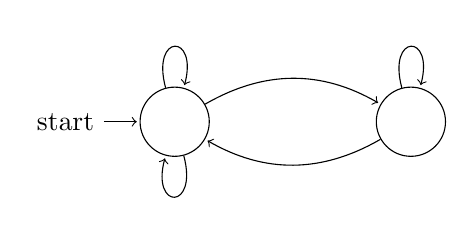
\begin{tikzpicture}[shorten >=1pt,node distance=1.5cm,on grid,auto]
\node[state, initial] (qI) at (-3,0) {};
\node[state] (qM) at (0,0) {};

\path[->] 
    (qI) edge [loop above] node {} (qI)
    (qI) edge [loop below] node {} (qI)
    (qI) edge [bend left] node {} (qM)
    (qM) edge [loop above] node {} (qM)
    (qM) edge [bend left] node {} (qI);
\end{tikzpicture}
\caption{An example of an \wB-automaton .}
\label{fig:wB}
\end{figure}


Consider the \wB-automaton  depicted on Figure~\ref{fig:wB}.  guesses (by moving to the state ) to measure the length of some blocks of letters . It accepts an -word  if and only if it is of the form


We can also treat  as an \wS-automaton. In that case the language recognised by  is

\end{example}

It is easy to check that a nondeterministic B\"uchi automaton can be transformed into an equivalent \wB- (resp. \wS)-automaton. Therefore, all -regular languages are both \wB- and \wS-regular.


\subsection{\fB- and \fS-automata} In the finite word models the situation is a little more complicated than in the \wB- and \wS-automata models. The automaton not only accepts or rejects a given word but also it assigns a \emph{value} to a word.

Formally, a \emph{\fT-automaton} (for ) is a counter automaton that is additionally equipped with a set of final states . An accepting run  of an automaton over a finite word  is a sequence of transitions starting in some initial state in  and ending in some final state in .

The following equations define  --- the value assigned to a given finite word by a given automaton. We use the convention that if a set of values is empty then the minimum of this set is  and the maximum is . The variable  ranges over all accepting runs,  ranges over counters in , while  ranges over positions where the counter  is reset in . As noted at the beginning of this section, we do not allow explicit \emph{check} operation, we only care about the values of the counters before resets.

\begin{description}
\item[\fB-automaton ] 
\item[\fS-automaton ] 
\end{description}

The following simple observation is crucial in the subsequent definitions.

\begin{lemma}\label{lm:val_regular}
For a given number , a \fB-automaton , and an \fS-automaton  the following languages of finite words are regular:

\end{lemma}

\begin{proof}
We can encode a bounded valuation of the counters into a state of a finite automaton.
\end{proof}

\subsection{Languages}

The above definitions give a semantics of a \fT-automaton in terms of a function . As noted in~\cite{torunczyk_limitedness}, it is possible to define the language recognised by such an automaton as a subset of the profinite monoid . We successively define it for \fB-automata and \fS-automata. In both cases the construction is justified by Lemma~\ref{lm:val_regular}.

{\bf \fB case:} Fix a \fB-automaton  and define


{\bf \fS case:} Fix an \fS-automaton  and define


\noindent Note that the sequences of languages in the above equations are monotone: increasing in \eqref{eq:def_B} and decreasing in \eqref{eq:def_S}.

\newcommand{\vfun}{\mathrm{val}_{\aut{A}}}

There exists another, equivalent way of defining languages recognised by these automata \cite{torunczyk_limitedness}. One can observe that the function  assigning to every finite word its value has a unique continuous extension on . The languages recognised by \fB- and \fS-automata can be defined as  and  respectively. In this work we only refer to the definitions \eqref{eq:def_B} and \eqref{eq:def_S}.

\begin{example}
Consider the \fS-automaton  depicted in Figure~\ref{fig:S}. The automaton measures the number of letters  in a given word. Then it guesses that the word is finished and moves to the accepting state. For every finite word  the value  equals the number of letters  in .

The language  does not contain any finite word. It contains a profinite word  if for every  the word  belongs to the profinite-regular language defined by the formula ``the word contains more than  letters '' (i.e. ). In particular, the limit of the sequence  from Example~\ref{ex:factorial} belongs to .

\begin{figure}
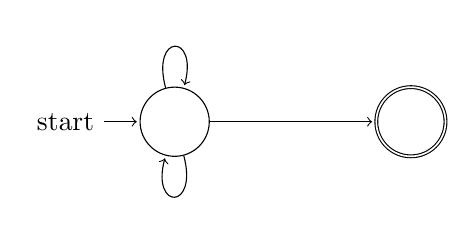
\begin{tikzpicture}[shorten >=1pt,node distance=1.5cm,on grid,auto]
\node[state, initial] (qI) at (-3,0) {};
\node[state, accepting] (qF) at (0,0) {};

\path[->] 
    (qI) edge [loop above] node {} (qI)
    (qI) edge [loop below] node {} (qI)
    (qI) edge [] node {} (qF);
\end{tikzpicture}
\caption{An example of an \fS-automaton .}
\label{fig:S}
\end{figure}
\end{example}

\begin{lemma}\label{lm:open_closed}
Every \fB-regular language is an open subset of \prom{A} and dually every \fS-regular language is closed.
\end{lemma}

\begin{proof}
By equations~\eqref{eq:def_B} and~\eqref{eq:def_S}, a \fB-regular language is a sum of profinite-regular languages and an \fS-regular language is an intersection of profinite-regular languages. By Fact~\ref{ft:clopen}, profinite-regular languages are closed and open, therefore their sum is open and the intersection is closed.
\end{proof}

The converse of Lemma~\ref{lm:open_closed} is false as there are uncountably many open subsets of \prom{A}.

We finish the definitions of automata models by recalling the following theorem.

\begin{theorem}[Fact~2.6 and Corollary~3.4 in~\cite{bojanczyk_bounds}, Theorem~8 and paragraph \emph{Closure properties} in~\cite{torunczyk_limitedness}]\label{th:effective_disjoint}

Let . The class of \fT-regular languages is effectively closed under union and intersection. The emptiness problem for \fT-regular languages is decidable.

Therefore, it is decidable whether given two \fT-regular languages are disjoint.
\end{theorem}



\section{Separation for profinite languages}\label{s:profinite_sep}

In this section we show the following theorem.

\begin{theorem}\label{th:separation}
Let . Assume that the languages of profinite words  are recognised by \fT-automata and . Then there exists a profinite-regular language  such that

\end{theorem}

The proof of the theorem consists of two parts, for the two cases of : Lemma~\ref{lm:s_separation} and Theorem~\ref{th:b_separation}.

First we prove the case when . The presented proof uses a general topological fact: the separation property of closed (i.e. ) sets in a zero-dimensional Polish space.

\begin{lemma}\label{lm:s_separation}
A pair of disjoint \fS-regular languages of profinite words can be separated by a profinite-regular language.
\end{lemma}

\begin{proof}
Take two \fS-regular languages .

Since  is a zero-dimensional Polish space, the -separation property holds for  (see Theorem~22.16 in~\cite{kechris_descriptive}). By Lemma~\ref{lm:open_closed} every \fS-regular language is  in , therefore  can be separated in  by a set  that is closed and open. By Fact~\ref{ft:clopen}, the language  is profinite-regular.
\end{proof}

Instead of using the -separation property, one can provide the following straightforward argument that uses the compactness of . We know that  is a closed subset of a compact space  so  is itself compact. Assume that  is recognised by an \fS-automaton . By \eqref{eq:def_S} we obtain


For  define  ---  the complement of the profinite-regular language . Clearly  because  and  are disjoint. Fact~\ref{ft:clopen} and Lemma~\ref{lm:val_regular} imply that the sets  are open subsets of . Therefore, the family  is an open cover of . Since  is compact, there is  such that


Therefore,  is a profinite-regular language that separates  and .

\begin{remark}\label{rm:effect_S}
The language  can be computed effectively.
\end{remark}

\begin{proof}
It is enough to observe that  can be taken as the minimal  such that  does not intersect the profinite-regular language . Such  exists by the above argument.
\end{proof}

Now we proceed with the separation property for \fB-regular languages. By Lemma~\ref{lm:open_closed} we know that \fB-regular languages are open sets in . An easy exercise shows that in general open sets do not have the separation property. Thus, to show the following theorem we need an argument that is a bit more involved than in the case of \fS-regular languages.

\begin{theorem}\label{th:b_separation}
A pair of disjoint \fB-regular languages of profinite words can be separated by a profinite-regular language.
\end{theorem}

We obtain the above theorem by applying the following observation.

\begin{lemma}\label{lm:closed}
For every \fB-regular language  there exists a profinite-regular language  such that


Moreover, the language  can be computed effectively.
\end{lemma}

\begin{proof}
Take a \fB-automaton  recognising . Define a new automaton  by removing from  all the counters and all the counter operations. What remains are transitions, initial states, and final states. Put . Of course  by the definition of . Clearly  by Theorem~\ref{th:iso}. What remains to show is that . 

Take a finite word . Observe that  has an accepting run on  because . So  because  cannot do more increments than the number of positions of the word. Therefore .
\end{proof}

\begin{proof}[Proof of Theorem~\ref{th:b_separation}]
Take two disjoint \fB-regular languages . Define  to be the language  from Lemma~\ref{lm:closed} for . Thus we know that . We only need to show that . Assume the contrary, that . Since \fB-regular languages are open sets in ,  is an open set. Since  is dense in  so  contains a finite word . But by the definition of  in that case . So  --- a contradiction to the disjointness of .
\end{proof}

\begin{remark}\label{rm:effect_prof}
Both separation results for \fB- and \fS-regular languages are effective: there is an algorithm that inputs two counter automata, verifies that the intersection of the languages is empty, and outputs an automaton recognising a separating language.
\end{remark}

\begin{proof}
By Theorem~\ref{th:effective_disjoint} it is decidable if two \fB- (resp. \fS)-regular languages are disjoint. As observed in Remark~\ref{rm:effect_S} and Lemma~\ref{lm:closed}, both constructions can be performed effectively.
\end{proof}



\section{Reduction}\label{s:reduction}

This section contains a proof of our crucial technical tool --- Theorem~\ref{th:recognition}. It is inspired by the \emph{reduction theorem} from~\cite{torunczyk_limitedness}.

Intuitively, \wB- and \wS-automata are composed of two \emph{orthogonal} parts, we can call them the -regular part and the asymptotic part. The -regular part corresponds to states and transitions of the automaton, while the asymptotic part represents quantitative conditions that can be measured by counters. In this section we show how to formally state this division. It can be seen as an extension of the technique presented in~\cite{bojanczyk_bounds}.

\begin{theorem}\label{th:recognition}
Fix an -automaton  and a type  in the trace monoid . There exists a \fT-regular language of profinite words  with the following property:

If  is an -word and  is a decomposition of  of type  then the following conditions are equivalent:
\begin{enumerate}
\item ,\label{it:in_lang}
\item there exists a grouping  of  that strongly converges to a profinite word ,\label{it:strongly_conv}
\item there exists a grouping  of  that converges to a profinite word .\label{it:conv}
\end{enumerate}

Additionally, one can ensure that . The construction of a \fT-automaton recognising  is effective given  and .
\end{theorem}

The rest of this section is devoted to showing the above theorem. We fix for the whole proof an \wT-automaton  and a type  in .

Intuitively, the requirement for a decomposition  to be of the type  corresponds to the -regular part of  while the convergence of  to an element of  takes care of the asymptotic part of .

Let us put  and assume that  is a deterministic finite automaton recognising the regular language . We will ensure that .

First we show how to construct a language , later we prove its properties. The definition of  depends on whether  or . The first case is a bit simpler.

{\bf Case } The language  is obtained as the union of finitely many \fB-regular languages indexed by states :

for \fB-automata  that we describe below. Intuitively, an automaton  measures \emph{loops} in  starting and ending in .

If for no  we have  or if  then . Assume otherwise. First we give an informal definition of :
\begin{itemize}
\item it is obtained from  by interpreting it as a finite word \fB-automaton,
\item it has initial and final state set to ,
\item it checks that all the counters are reset in a given word,
\item it checks that a given word belongs to ,
\item it resets all the counters at the end of the word.
\end{itemize}

Now we give a precise definition of . 
Let:
\begin{itemize}
\item ,
\item ,
\item ,
\item ,
\end{itemize}
and let  contain the following transitions:
\begin{itemize}
\item  if ,  and for every  we have ,
\item  for  if .
\end{itemize}

The state  is the only final state used to perform the reset at the end of a word. During a run, the automaton  simulates  and  in parallel, using  and . Additionally, a vector in  denotes for every counter whether it was already reset in a word or not.

{\bf Case } In that case the language  is obtained as the union of finitely many \fS-regular languages indexed by pairs :

Intuitively, an automaton  recognises loops  as before. Additionally, the vector  denotes whether a given counter  obtains bigger values before the first reset () or after the last reset () on a given finite word. The following definition formalises this property. A similar technique of assigning a \emph{reset type} to a finite run can be found in~\cite{bojanczyk_bounds}.

\begin{definition}\label{def:etype}
Let  be a run of some counter automaton  over an -word . Let  be a position in  and let  be a counter of . Let:

\begin{itemize}
\item  be the number of increments of  between the last reset before  and ,
\item  be the number of increments of  between  and the first reset after .
\end{itemize}
If there is no reset of  at some side of  then the respective value is . Define the \emph{end-type} of  on  in  (denoted as ) by the following equation:


\end{definition}

As before if for no , we have  or if  then . Assume otherwise. We start with an informal definition of :
\begin{itemize}
\item it is obtained from  by interpreting it as a finite word \fS-automaton,
\item it has initial and final state set to ,
\item it checks that all the counters are reset in a given word,
\item it checks that a given word belongs to ,
\item for every counter :
\begin{itemize}
\item if  then  skips the first reset of  and all the previous increments of  but resets  at the end of a given word,
\item if  then  acts on  exactly as  (with no additional reset at the end of the word).
\end{itemize}
\end{itemize}

Formally, let  such that
\begin{itemize}
\item ,
\item ,
\item ,
\item ,
\end{itemize}
and  contains the following transitions:
\begin{itemize}
\item  if , , and for every  we have:
\begin{itemize}
\item ,
\item if  and  then , otherwise ,
\end{itemize}
\item  if  and for every  we have  if  and  otherwise.
\end{itemize}

\noindent Now we proceed with the proof that the above constructions give us the desired language . First note that in both cases the constructed automata explicitly verify that a given word belongs to . Therefore, .

We start by taking an -word  and its decomposition  of the type .

\subsection{Implication }

Assume that there exists an accepting run  of  over . We want to construct a grouping  of  such that:
\begin{enumerate}[label=S.\arabic*]
\item for  we have ,\label{en:type}
\item all counters in  are reset by  in every word ,\label{en:counters}
\item the state that occurs in the run  at the end-points of all the words  is some fixed state ,\label{en:state}
\item there exists a vector  such that for every counter  and every position  between successive words  in  we have ,\label{en:vector}
\item the sequence of words  is strongly convergent to some profinite word .\label{en:conv}
\end{enumerate}

The grouping  is obtained in steps. Observe that all the above properties are preserved when taking a grouping of a sequence. \ref{en:type} is already satisfied by the sequence . First, we group words of  in such a way to satisfy \ref{en:counters} using the fact that the run  is accepting. Then we further group the sequence to satisfy \ref{en:state} and \ref{en:vector} --- some state and value of  must appear in infinitely many end-points. Finally, we apply Theorem~\ref{th:ramsey_compact} to group the sequence into a strongly convergent one. 

Now, it suffices to show that . First, observe that  is a witness that there is a path from  to  and from  to  in .

We consider two cases:
\begin{description}
\item[\bf Case ] Since  is accepting, there exists a constant  such that the values of all counters during  are bounded by . We show that for every  we have . It implies that  and therefore .

Observe that  induces a run  of  on . By \ref{en:type}, \ref{en:counters}, and \ref{en:state} we know that  is an accepting run of  --- it starts in the only initial state and ends in . Since  simulates all the resets of , we know that  and therefore .

\item[\bf Case ] We show that for every  the sequence  from some point on satisfies . It implies that for every  we have  and therefore .

Since  is accepting, for every constant , from some point on, all the counters are reset with a value greater than . Assume that the last reset with the value at most  occurs before the word . We show that for  we have . Let  be the sequence of transitions of  on . Observe that  induces a run  of  on . As before,  is accepting by \ref{en:type}, \ref{en:state}, and \ref{en:counters}. Take a counter  and a reset of this counter  in . Consider the following cases, recalling Definition~\ref{def:etype}:

\begin{itemize}
\item  corresponds to the first reset of  in the run . Since  did not skip , . Therefore,  has more increments after the beginning of  than before it in . Therefore .
\item  corresponds to a reset of  in the run  but not the first one. In that case .
\item  is the additional reset performed by  at the end of the word . In that case  so  has greater or equal number of increments before the end of the word  than after it in . Therefore .
\end{itemize}

In all three cases . So we have shown that

\end{description}

\subsection{Implication }

This implication is trivial since strong convergence entails convergence.

\subsection{Implication }

Let  be a grouping of  such that  converges to a limit .

We consider two cases:
\begin{description}
\item[\bf Case ] Since , there exists a state  such that . Therefore,  for some . Since  is an open set and  is a limit of , almost all elements of  belong to . Assume that for  we have . Let  be a run that witnesses this fact. By the construction of , the run  induces a run  of  on . Also, since  is accepting,  resets all the counters at least once.

By the assumption about , there exists a run  of  on  that starts in some state in  and ends in , and a sequence of runs  on  for  that lead from  to . Therefore, we can construct an infinite run  of  on  being the concatenation of the runs  on the words  for . We show that if  is a reset of a counter  in  that appears after the word  then . Since there are only finitely many resets of counters before the word , this bound suffices to show that the run  is accepting.

Observe that the increments in  correspond to the increments in the runs . Also,  performs all the resets that appear in runs  except the resets at the end of the words. There can be at most one such skipped reset in a row because every counter is reset in every run . Therefore, .



\item[\bf Case ] Let  be parameters such that . Therefore, for every  we have . As  is convergent to  and languages  are open, it means that


As above we construct a run  over  that first leads on  from some state of  to  and later consists of a concatenation of runs over words . Let  be any run of  that leads from  to  on . For  we pick a run  in such a way that it is accepting and\footnote{Since there are only finitely many runs of an automaton on a finite word, there always exists a run realising the value , no matter whether the value is finite or not.}

Observe that by \eqref{eq:limits}, we obtain


For  by  be denote the run of  on  induced by . Similarly as in the previous case, runs  for  can be combined into a run  of  on . By the construction of ,  resets every counter infinitely often.

Let  be a position in  where a counter  is reset during . Assume that  is contained in a word  and  --- we do not care about first two words.

Consider two cases:
\begin{description}
\item[] In that case  performs the same increments and resets of  as the runs . Therefore, .
\item[] If  is not the first reset of  in  then the value of  before  in  is the same as in . Assume that  is the first reset of  in . Note that  performs an additional reset of  at the end of . This reset does not appear in  so .
\end{description}

In all the cases

so the values of  before successive resets tend to infinity by \eqref{eq:tends}. It means that  is an accepting run and .
\end{description}



\section{Separation for -languages}\label{s:omega_sep}

In this section we show the main result of the paper. The technique is to lift the separation results for \fT-regular languages of profinite words into the -word case.

\begin{theorem}\label{th:main}
Let . If  are disjoint languages of -words both recognised by \wT-automata then there exists an -regular language  such that


Additionally, the construction is effective.
\end{theorem}

The rest of the section is devoted to showing this theorem. As observed by Thomas Colcombet, in the case of  the thesis can be proved directly, without referring to profinite words. This simpler proof is presented in Section~\ref{s:direct} with his kind permission. However, the  case is also treated here for two reasons: first it reveals the symmetry and generality of the ``profinite approach'', second it can be used as a guideline for the more complex case of .

Let  and  denote the trace-monoid for an \wT-automaton  recognising . Let  be the canonical homomorphisms from  to . Define  as the set of types  in the trace-monoid .

For every type  define  as the \fT-regular language of profinite words given by Theorem~\ref{th:recognition} for  and . By the statement of the theorem we know that .

\begin{definition}
For a pair of types , we say that  are \emph{coherent} if there exist finite words  such that:  and  for .
\end{definition}

An important application of Theorem~\ref{th:recognition} is the following lemma.

\begin{lemma}
If a pair of types  is coherent then the languages  are disjoint.
\end{lemma}

\begin{proof}
Take coherent types  and .

Assume that there exists a profinite word . Since  for , there exists a sequence  of finite words converging to  such that  and  for all . Moreover, by coherency of  there exists a finite word  such that  and . Let  We show that  --- a contradiction.

Take . Observe that  is a decomposition of  of -type . Additionally observe that the sequence  converges to  and  belongs to . So, by Theorem~\ref{th:recognition} we have .
\end{proof}

Take a pair of coherent types . Since the languages  are disjoint, we can use Theorem~\ref{th:separation} to find a separating profinite-regular language  such that


Now we can introduce the -regular language  separating .

\begin{definition}
Consider a coherent pair of types . Let  be defined as follows:  is the language of -words  such that there exists a decomposition  of types  with respect to , such that every grouping of  from some point on belongs to the regular language .

Note that the above definition can be expressed in MSO so  is an -regular language.

Let  be the -regular language defined as

where the sum ranges over pairs of coherent types.
\end{definition}

Clearly  is an -regular language. What remains is to show the following lemma.

\begin{lemma}
The language  separates  and .
\end{lemma}

\begin{proof}
First observe that . Take . We want to construct a decomposition  of  such that:
\begin{itemize}
\item the -type of  is  for  and some pair of coherent types  in ,
\item the sequence  is strongly convergent to some profinite word .
\end{itemize}

The sequence  is obtained in steps. First we use Theeorem~\ref{th:ramsey} to find a decomposition of  with respect to both monoids  at the same time. Such decomposition satisfies the first bullet above. Then, using Theorem~\ref{th:ramsey_compact}, we can group our sequence into  in such a way that  is strongly convergent.

By Theorem~\ref{th:recognition}, there exists a grouping  of  that converges to a profinite word . But since  is strongly convergent, . Therefore, by the strong convergence of , every grouping of  converges to . So every grouping of  from some point on belongs to  as in the definition of . Therefore, .

Now we show that . Assume otherwise, that there exists an -word . Since , there exists a coherent pair of types  such that . Therefore,  can be decomposed as  of types  respectively. Let  Because  so by Theorem~\ref{th:recognition} there exists a grouping  of  with a limit  . But by the definition of  almost all words in  belong to  so . Since , we have the required contradiction.
\end{proof}

Now we can deduce the corollary from the introduction.

\begin{corollary}\label{cl:delta}
If a given language of -words  and its complement  are both \wB-regular (resp. \wS-regular) then  is (effectively) -regular.
\end{corollary}

\begin{proof}
Let  be a language of -words such that  and  are both -regular. By Theorem~\ref{th:main} there exists an -regular language  that separates  and . But in that case  so  is -regular.
\end{proof}



\section{A direct proof of separation for \wB-regular languages}\label{s:direct}

As observed by Thomas Colcombet, the separation property for \wB-regular languages can be shown directly, without referring to profinite words. This simpler proof is presented here with his kind permission.

Let  be an \wB-regular language recognised by an \wB-automaton . Consider a B\"uchi automaton  obtained from  by removing all the counter operations (similarly to Lemma~\ref{lm:closed}) and requiring that every counter is reset infinitely often.

Clearly, the language recognized by  is -regular and .

\begin{claim}\label{cl:ultimat}
If  is an ultimately periodic -word in  then .
\end{claim}

\begin{proof}
Observe that  has an ultimately periodic accepting run  on . By the acceptance condition of , every counter  of  is reset infinitely often during . Since  is ultimately periodic, the values of the counter  are bounded in . Therefore, .
\end{proof}

It means that, since an -regular language is entirely defined by the ultimately periodic -words it contains~\cite{buchi_decision},  is the least -regular language that contains . It also means that it depends only on  but not on the specific automaton  that recognizes it. Let us call this language .

Consider now two \wB-regular languages of empty intersection  and . Assume  intersects  then, since these languages are -regular, there is an ultimately periodic -word in this intersection. But according to Claim~\ref{cl:ultimat}, this ultimately periodic -word belongs to both  and . A contradiction.

It follows that if  and  are disjoint then  (respectively ) are separators. Also, this construction shows that in order to construct a separator of two \wB-regular languages, only one language needs to be known.



\section{Acknowledgements}\label{s:ack}

The author would like to thank Miko{\l}aj Boja{\'n}czyk for his suggestions. This paper makes noticeable use of results by Szymon Toru{\'n}czyk: his PhD thesis~\cite{torunczyk_phd} and paper~\cite{torunczyk_limitedness}. The author would like to thank Filip Mazowiecki and the referees for careful reading the text and providing a number of important comments. Moreover, Thomas Colcombet had a gainful influence on the paper by providing a direct proof for the separation of \wB-regular languages.



\bibliographystyle{alpha}
\bibliography{mskrzypczak}

\end{document}
